\begin{table}[h]
\centering
\begin{minipage}{0.48\linewidth}
    \caption{Comparison of Transformer-based methods on EuRoC dataset and BlackBIrd dataset. Evaluation metric: ATE (Unit: \si{\meter}) and RTE (Unit: \si{\meter})}
    \label{tab:airio:transformer_euroc}
    \centering
\resizebox{0.5\linewidth}{!}{
    \begin{tabular}{C{2cm}|C{.8cm}C{.8cm}C{.8cm}C{.8cm}C{.8cm}C{.8cm}C{.8cm}C{.8cm}}
        \toprule
        \multirow{2}{*}
        {\textbf{Seq.}}&  \multicolumn{2}{c}{\multirow{2}{*}{\shortstack{\textbf{Transformer} \\ \textbf{$+$Global}}}} &  \multicolumn{2}{c}{\multirow{2}{*}{\shortstack{\textbf{Transformer} \\ \textbf{$+$Body}}}} &  \multicolumn{2}{c}{\multirow{2}{*}{\shortstack{\textbf{Transformer} \\ \textbf{$+$Attitude}}}} &  \multicolumn{2}{c}{\multirow{2}{*}{\textbf{AirIO Net}}}\\ 
        & & & & & &&&\\
        &  ATE  &  RTE &  ATE  &  RTE &  ATE  &  RTE &  ATE  &  RTE\\
        \midrule
        \raggedright \textbf{EuRoC}  & \multicolumn{2}{c}{} & \multicolumn{2}{c}{} & \multicolumn{2}{c}{} & \multicolumn{2}{c}{}\\

         MH02 &\cellcolor{g7!100} 12.03 & \cellcolor{g7!100} 2.995 & \cellcolor{g5!100} 3.357 & \cellcolor{g5!100} 1.081 & \cellcolor{g1!100} \textbf{2.452} & \cellcolor{g1!100}\textbf{0.885} & \cellcolor{g3!100} 2.531 & \cellcolor{g3!100} 0.972 \\
         
         MH04 &\cellcolor{g7!100} 11.964 & \cellcolor{g7!100} 7.395 & \cellcolor{g5!100} 4.764 & \cellcolor{g5!100} 1.159 & \cellcolor{g3!100} 2.306 & \cellcolor{g3!100} 1.096 & \cellcolor{g1!100} \textbf{2.25} & \cellcolor{g1!100} \textbf{1.009} \\

         
         V103 & \cellcolor{g7!100} 9.93 & \cellcolor{g7!100} 2.932 & \cellcolor{g5!100} 7.624 & \cellcolor{g3!100} 1.46 & \cellcolor{g3!100} 4.978 & \cellcolor{g1!100} \textbf{1.445} & \cellcolor{g1!100} \textbf{3.107} & \cellcolor{g5!100} 1.512 \\


         
         V202 &\cellcolor{g7!100} 10.689 & \cellcolor{g7!100} 3.057 & \cellcolor{g1!100} \textbf{2.521} & \cellcolor{g1!100} \textbf{1.042} & \cellcolor{g5!100} 5.567 & \cellcolor{g3!100} 1.23 & \cellcolor{g3!100} 4.31 & \cellcolor{g5!100} 1.263 \\

         V101 &\cellcolor{g5!100} 10.322 & \cellcolor{g7!100} 2.276 & \cellcolor{g7!100} 15.762 & \cellcolor{g5!100} 1.472 & \cellcolor{g3!100} 6.673 & \cellcolor{g3!100} 1.303 & \cellcolor{g1!100} \textbf{4.287} & \cellcolor{g1!100} \textbf{1.104} \\
        \textbf{Avg.} &\cellcolor{g7!100} 10.987 & \cellcolor{g7!100} 3.731 & \cellcolor{g5!100} 6.806 & \cellcolor{g5!100} 1.243 & \cellcolor{g3!100} 4.395 & \cellcolor{g3!100} 1.192 & \cellcolor{g1!100} \textbf{3.297} & \cellcolor{g1!100} \textbf{1.172} \\

        \midrule
        \midrule
    \raggedright \textbf{BB. Seen}  & \multicolumn{2}{c}{} & \multicolumn{2}{c}{} & \multicolumn{2}{c}{} & \multicolumn{2}{c}{}\\

    clover &\cellcolor{g7!100} 0.983 & \cellcolor{g7!100} 0.714 & \cellcolor{g3!100} 0.481 & \cellcolor{g3!100} 0.379 & \cellcolor{g5!100} 0.645 & \cellcolor{g5!100} 0.389 & \cellcolor{g1!100} \textbf{0.411} & \cellcolor{g1!100} \textbf{0.355} \\
    
   halfMoon &\cellcolor{g7!100} 0.48 & \cellcolor{g5!100} 0.23 & \cellcolor{g3!100} 0.223 & \cellcolor{g1!100} \textbf{0.129} & \cellcolor{g1!100} \textbf{0.219} & \cellcolor{g3!100} 0.219 & \cellcolor{g5!100} 0.445 & \cellcolor{g7!100} 0.243 \\
   
 star &\cellcolor{g7!100} 1.323 & \cellcolor{g7!100} 2.053 & \cellcolor{g5!100} 0.955 & \cellcolor{g5!100} 0.586 & \cellcolor{g1!100} \textbf{0.401} & \cellcolor{g3!100} 0.469 & \cellcolor{g3!100} 0.43 & \cellcolor{g1!100} \textbf{0.346} \\
 
egg&\cellcolor{g3!100} 0.698 & \cellcolor{g5!100} 0.521 & \cellcolor{g5!100} 0.914 & \cellcolor{g3!100} 0.479 & \cellcolor{g7!100} 1.013 & \cellcolor{g7!100} 0.79 & \cellcolor{g1!100} \textbf{0.677} & \cellcolor{g1!100} \textbf{0.356} \\

 winter&\cellcolor{g7!100} 0.856 & \cellcolor{g7!100} 0.548 & \cellcolor{g1!100} \textbf{0.276} & \cellcolor{g3!100} 0.215 & \cellcolor{g5!100} 0.386 & \cellcolor{g5!100} 0.325 & \cellcolor{g3!100} 0.359 & \cellcolor{g1!100} \textbf{0.165} \\

\textbf{Avg.} & \cellcolor{g7!100} 0.868 & \cellcolor{g7!100} 0.813 & \cellcolor{g5!100} 0.57 & \cellcolor{g3!100} 0.358 & \cellcolor{g3!100} 0.532 & \cellcolor{g5!100} 0.438 & \cellcolor{g1!100} \textbf{0.464} & \cellcolor{g1!100} \textbf{0.293} \\
    \midrule
    \midrule
\raggedright \textbf{BB. Unseen}  & \multicolumn{2}{c}{} & \multicolumn{2}{c}{} & \multicolumn{2}{c}{} & \multicolumn{2}{c}{}\\
ampersand &\cellcolor{g7!100} 11.4 & \cellcolor{g7!100} 4.417 & \cellcolor{g5!100} 3.112 & \cellcolor{g5!100} 1.954 & \cellcolor{g1!100} \textbf{1.931} & \cellcolor{g3!100} 1.428 & \cellcolor{g3!100} 2.492 & \cellcolor{g1!100} \textbf{1.185} \\

 sid&\cellcolor{g7!100} 3.932 & \cellcolor{g7!100} 5.765 & \cellcolor{g5!100} 1.564 & \cellcolor{g3!100} 0.842 & \cellcolor{g3!100} 0.824 & \cellcolor{g5!100} 0.847 & \cellcolor{g1!100} \textbf{0.651} & \cellcolor{g1!100} \textbf{0.504} \\
 
oval&\cellcolor{g7!100} 8.935 & \cellcolor{g7!100} 5.137 & \cellcolor{g3!100} 0.707 & \cellcolor{g1!100} \textbf{0.463} & \cellcolor{g1!100} \textbf{0.614} & \cellcolor{g5!100} 0.639 & \cellcolor{g5!100} 0.913 & \cellcolor{g3!100} 0.558 \\
 
sphinx&\cellcolor{g7!100} 3.778 & \cellcolor{g7!100} 4.971 & \cellcolor{g5!100} 1.396 & \cellcolor{g3!100} 1.164 & \cellcolor{g1!100} \textbf{1.139} & \cellcolor{g5!100} 1.78 & \cellcolor{g3!100} 1.164 & \cellcolor{g1!100} \textbf{1.022} \\
 
bentDice&\cellcolor{g7!100} 3.904 & \cellcolor{g7!100} 3.755 & \cellcolor{g5!100} 1.594 & \cellcolor{g3!100} 1.266 & \cellcolor{g3!100} 1.437 & \cellcolor{g5!100} 1.36 & \cellcolor{g1!100} \textbf{1.249} & \cellcolor{g1!100} \textbf{0.872} \\
 
\textbf{Avg.} & \cellcolor{g7!100} 6.39 & \cellcolor{g7!100} 4.809 & \cellcolor{g5!100} 1.675 & \cellcolor{g3!100} 1.138 & \cellcolor{g1!100} \textbf{1.189} & \cellcolor{g5!100} 1.211 & \cellcolor{g3!100} 1.294 & \cellcolor{g1!100} \textbf{0.828} \\

    
        \bottomrule
        % \multicolumn{9}{l}{$^\dagger$ Leverage ground truth orientation to transform the input data for inference.}\\

    \end{tabular}
    }
\end{minipage}
\hfill
\begin{minipage}{0.48\linewidth}
 \centering
    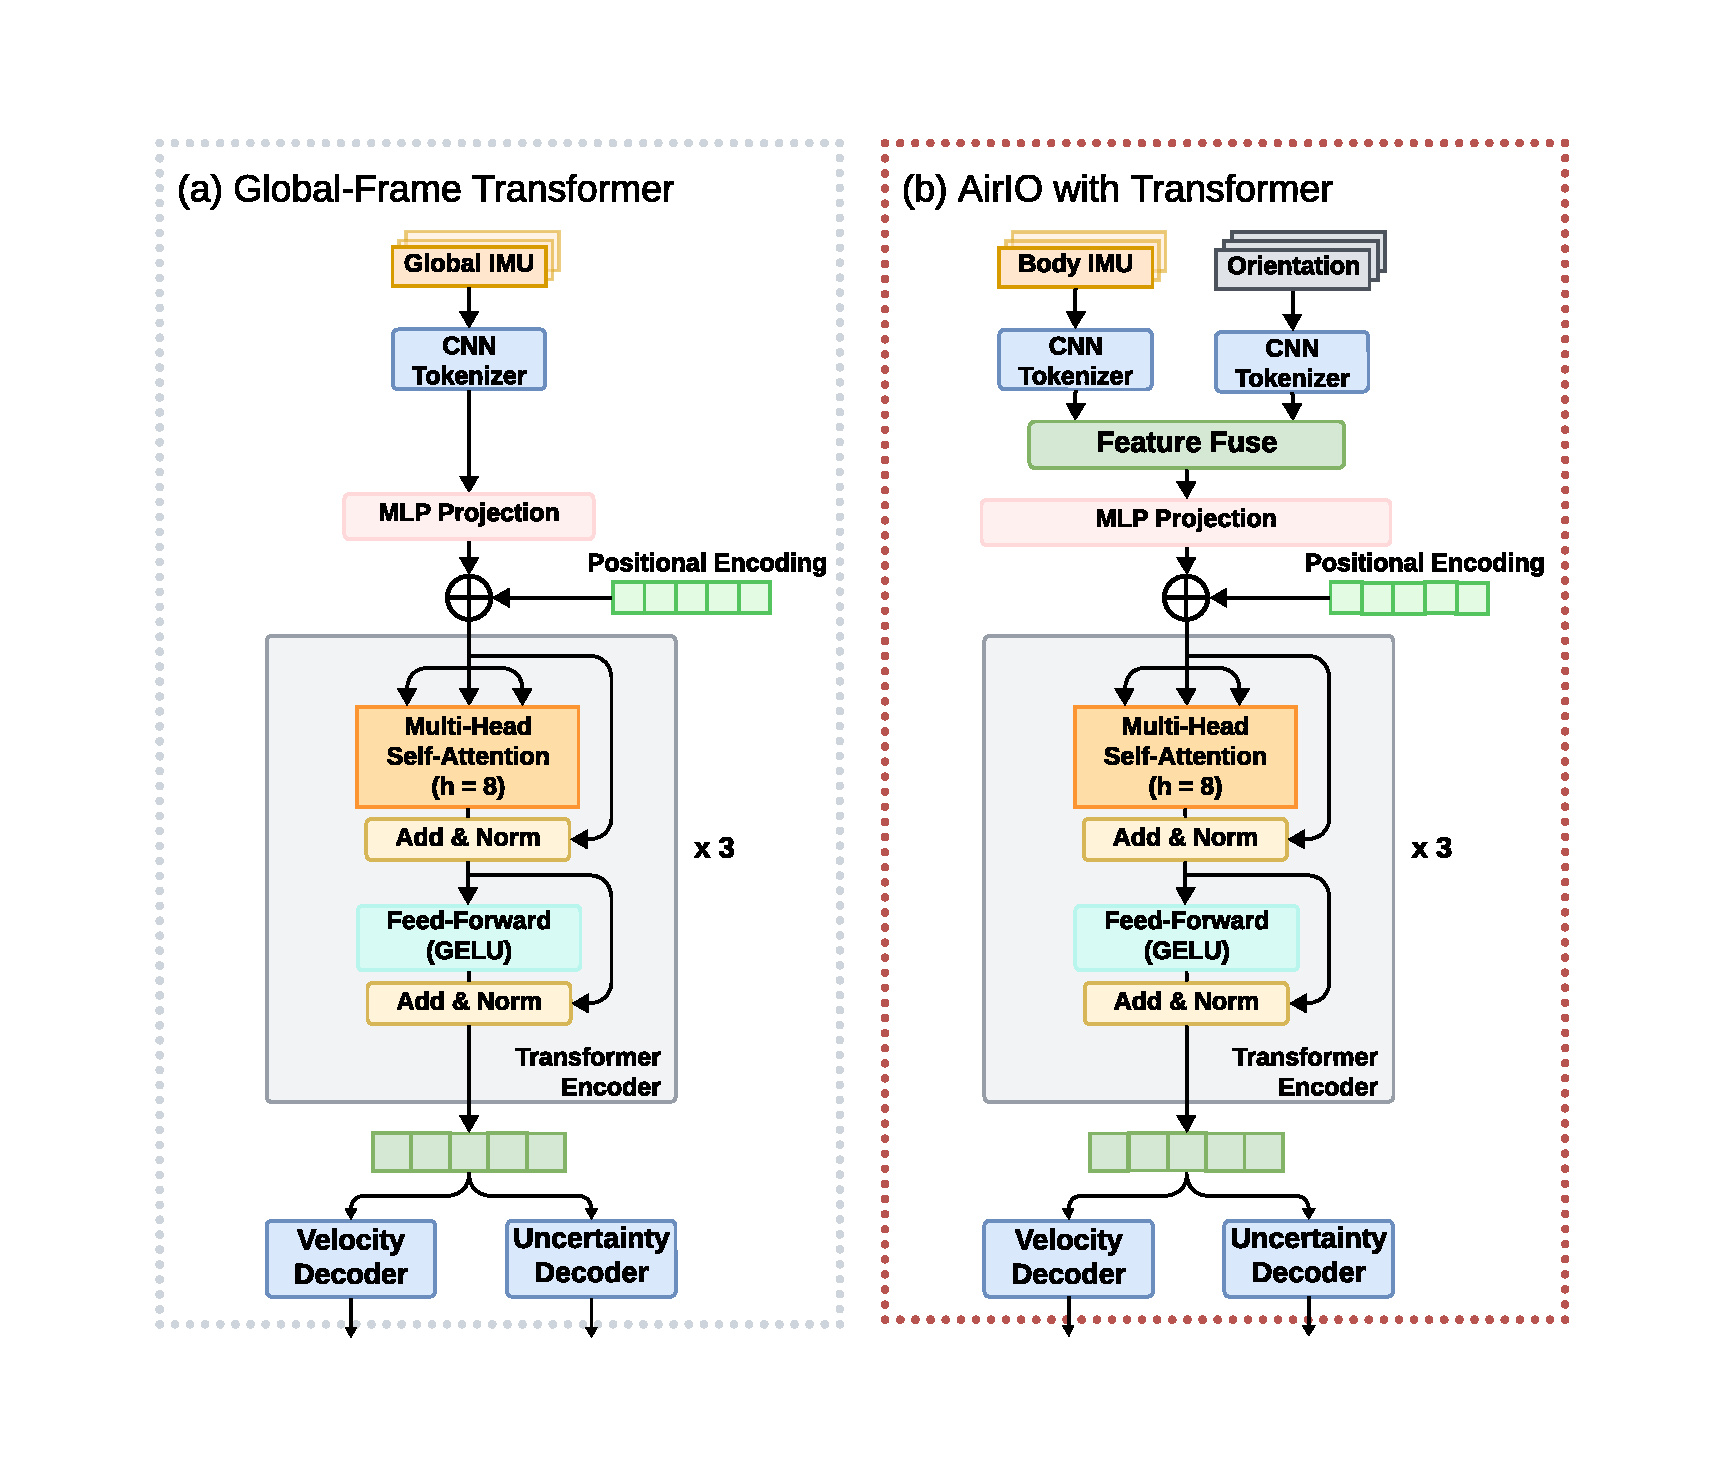
\includegraphics[width=0.5\linewidth]{tex/ch5_airio/figs/Transformer.pdf}
    \caption{Enter Caption}
    \label{fig:airio:transformer_arch}
\end{minipage}
\end{table}

